% Options for packages loaded elsewhere
\PassOptionsToPackage{unicode}{hyperref}
\PassOptionsToPackage{hyphens}{url}
\PassOptionsToPackage{dvipsnames,svgnames*,x11names*}{xcolor}
%
\documentclass[
  12pt,
]{article}
\usepackage{amsmath,amssymb}
\usepackage{lmodern}
\usepackage{ifxetex,ifluatex}
\ifnum 0\ifxetex 1\fi\ifluatex 1\fi=0 % if pdftex
  \usepackage[T1]{fontenc}
  \usepackage[utf8]{inputenc}
  \usepackage{textcomp} % provide euro and other symbols
\else % if luatex or xetex
  \usepackage{unicode-math}
  \defaultfontfeatures{Scale=MatchLowercase}
  \defaultfontfeatures[\rmfamily]{Ligatures=TeX,Scale=1}
\fi
% Use upquote if available, for straight quotes in verbatim environments
\IfFileExists{upquote.sty}{\usepackage{upquote}}{}
\IfFileExists{microtype.sty}{% use microtype if available
  \usepackage[]{microtype}
  \UseMicrotypeSet[protrusion]{basicmath} % disable protrusion for tt fonts
}{}
\makeatletter
\@ifundefined{KOMAClassName}{% if non-KOMA class
  \IfFileExists{parskip.sty}{%
    \usepackage{parskip}
  }{% else
    \setlength{\parindent}{0pt}
    \setlength{\parskip}{6pt plus 2pt minus 1pt}}
}{% if KOMA class
  \KOMAoptions{parskip=half}}
\makeatother
\usepackage{xcolor}
\IfFileExists{xurl.sty}{\usepackage{xurl}}{} % add URL line breaks if available
\IfFileExists{bookmark.sty}{\usepackage{bookmark}}{\usepackage{hyperref}}
\hypersetup{
  pdftitle={Supplemental Materials for ``Popularity Adjusted Block Models are Generalized Random Dot Product Graphs''},
  colorlinks=true,
  linkcolor=Maroon,
  filecolor=Maroon,
  citecolor=Blue,
  urlcolor=blue,
  pdfcreator={LaTeX via pandoc}}
\urlstyle{same} % disable monospaced font for URLs
\usepackage[margin=1in]{geometry}
\usepackage{graphicx}
\makeatletter
\def\maxwidth{\ifdim\Gin@nat@width>\linewidth\linewidth\else\Gin@nat@width\fi}
\def\maxheight{\ifdim\Gin@nat@height>\textheight\textheight\else\Gin@nat@height\fi}
\makeatother
% Scale images if necessary, so that they will not overflow the page
% margins by default, and it is still possible to overwrite the defaults
% using explicit options in \includegraphics[width, height, ...]{}
\setkeys{Gin}{width=\maxwidth,height=\maxheight,keepaspectratio}
% Set default figure placement to htbp
\makeatletter
\def\fps@figure{htbp}
\makeatother
\setlength{\emergencystretch}{3em} % prevent overfull lines
\providecommand{\tightlist}{%
  \setlength{\itemsep}{0pt}\setlength{\parskip}{0pt}}
\setcounter{secnumdepth}{5}
\usepackage{float}
\usepackage{mathtools}
\usepackage{natbib}
\usepackage[linesnumbered,ruled,vlined]{algorithm2e}
\setcitestyle{numbers,square,comma}
\usepackage{verbatim}
\usepackage{amsthm}
\usepackage{comment}
\ifluatex
  \usepackage{selnolig}  % disable illegal ligatures
\fi
\usepackage[]{natbib}
\bibliographystyle{plainnat}

\title{Supplemental Materials for ``Popularity Adjusted Block Models are
Generalized Random Dot Product Graphs''}
\author{}
\date{\vspace{-2.5em}}

\begin{document}
\maketitle

\newcommand{\diag}{\mathrm{diag}}
\newcommand{\tr}{\mathrm{Tr}}
\newcommand{\blockdiag}{\mathrm{blockdiag}}
\newcommand{\indep}{\stackrel{\mathrm{ind}}{\sim}}
\newcommand{\iid}{\stackrel{\mathrm{iid}}{\sim}}
\newcommand{\Bernoulli}{\mathrm{Bernoulli}}
\newcommand{\Betadist}{\mathrm{Beta}}
\newcommand{\BG}{\mathrm{BernoulliGraph}}
\newcommand{\PABM}{\mathrm{PABM}}
\newcommand{\RDPG}{\mathrm{RDPG}}
\newcommand{\GRDPG}{\mathrm{GRDPG}}
\newcommand{\Multinomial}{\mathrm{Multinomial}}

\hypertarget{sparsity-simulation-study}{%
\section{Sparsity Simulation Study}\label{sparsity-simulation-study}}

In this simulation study, we use the same setup as in the simulations
for balanced communities but with fixed \(K = 3\) and \(n = 2^{11}\) and
vary the sparsity parameter \(\rho \in (0, 1]\) (this was fixed at
\(\rho_n = 1\) for the previous simulations. More specifically,

\begin{itemize}
\tightlist
\item
  Number of vertices \(n = 2048\)
\item
  Number of underlying communities \(K = 3\)
\item
  Sparsity parameter \(\rho_n = 0.1, 0.3, 0.5, 0.7, 0.9\)
\item
  Mixture parameters \(\alpha_k = 1 / K\) for \(k = 1, ..., K\) (i.e.,
  each community label has an equal probability of being drawn)
\item
  Community labels
  \(z_k \stackrel{\mathrm{iid}}{\sim}\mathrm{Multinomial}(\alpha_1, ..., \alpha_K)\)
\item
  Within-group popularities
  \(\lambda^{(kk)} \stackrel{\mathrm{iid}}{\sim}\mathrm{Beta}(2, 1)\)
\item
  Between-group popularities
  \(\lambda^{(k \ell)} \stackrel{\mathrm{iid}}{\sim}\mathrm{Beta}(1, 2)\)
  for \(k \neq \ell\)
\end{itemize}

Fifty simulations were performed for each combination of \(n\) and
\(K\). The results for community detection and parameter estimation
error are shown in Fig. \ref{fig:sparsity_sim}. Community detection
error is defined as the number of misclustered vertices. Parameter
estimation error is defined as \(\frac{1}{n} \|P - \hat{P}\|_F\) where
\(\hat{P}\) is the estimated edge probability matrix.

\begin{figure}[H]

{\centering 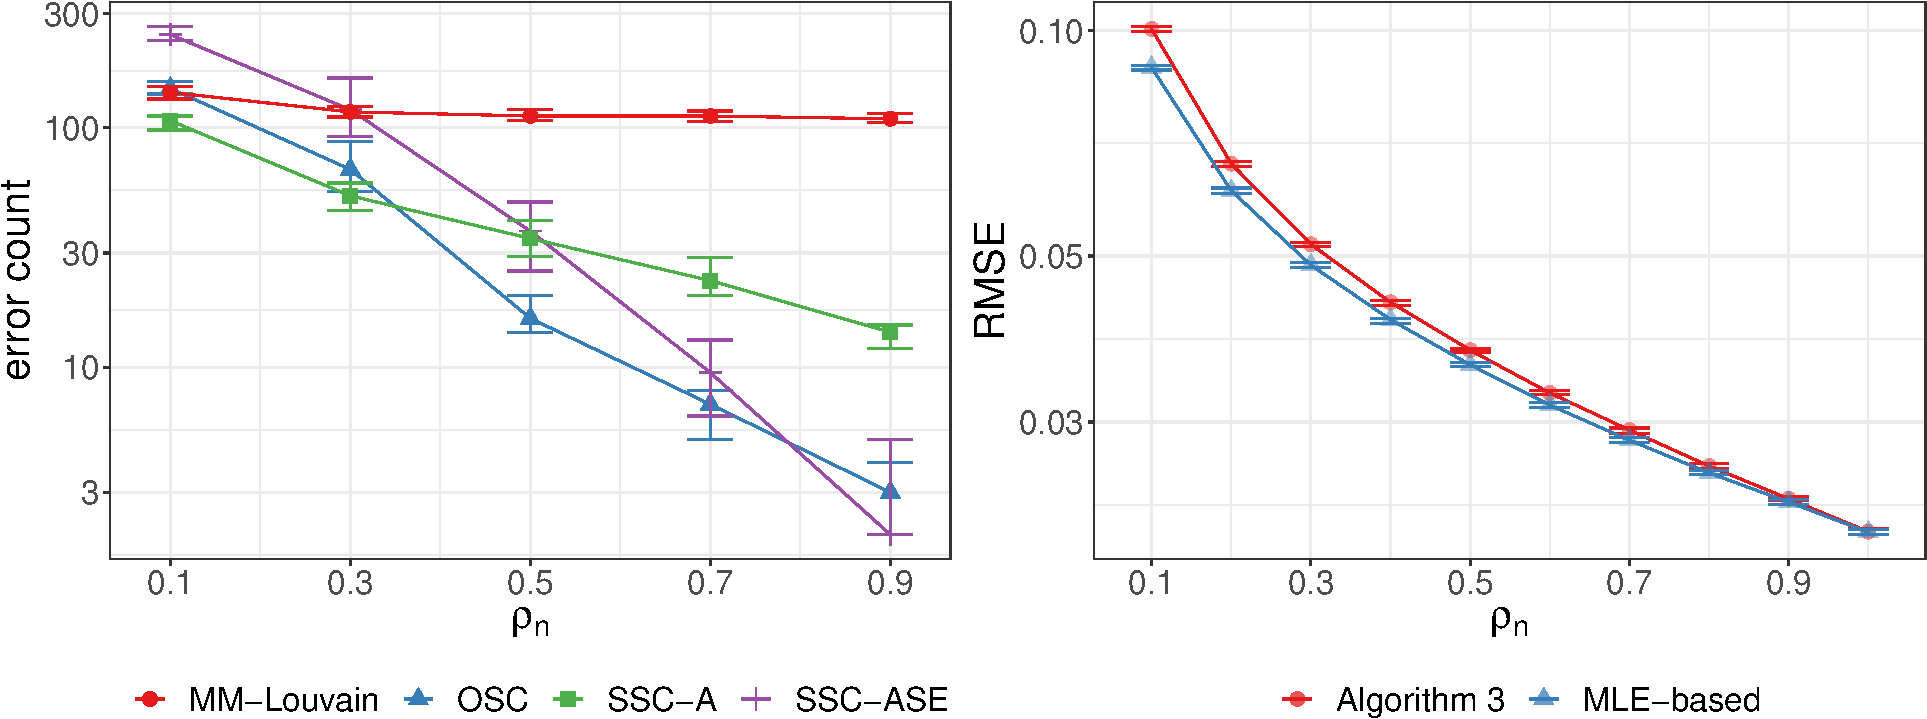
\includegraphics[width=1\linewidth]{supplemental-materials_files/figure-latex/sparsity_sim-1} 

}

\caption{Community detection error counts (left) and popularity parameter RMSEs (right) for $n = 2048$ and $K = 3$ and varying $\rho_n$. Simulations were repeated 50 times for each $\rho_n$.}\label{fig:sparsity_sim}
\end{figure}

\renewcommand\refname{Choice of \(\vartheta\) for the Subspace Detection
Property}
  \bibliography{misc.bib}

\end{document}
